 \addtolength\abovedisplayskip{-1\baselineskip}%
  \addtolength\belowdisplayskip{-1\baselineskip}%
 
\begin{tikzpicture}
\node (datatitle) {\small Raw Data};
\node[below = -0.25cm of datatitle] (data) {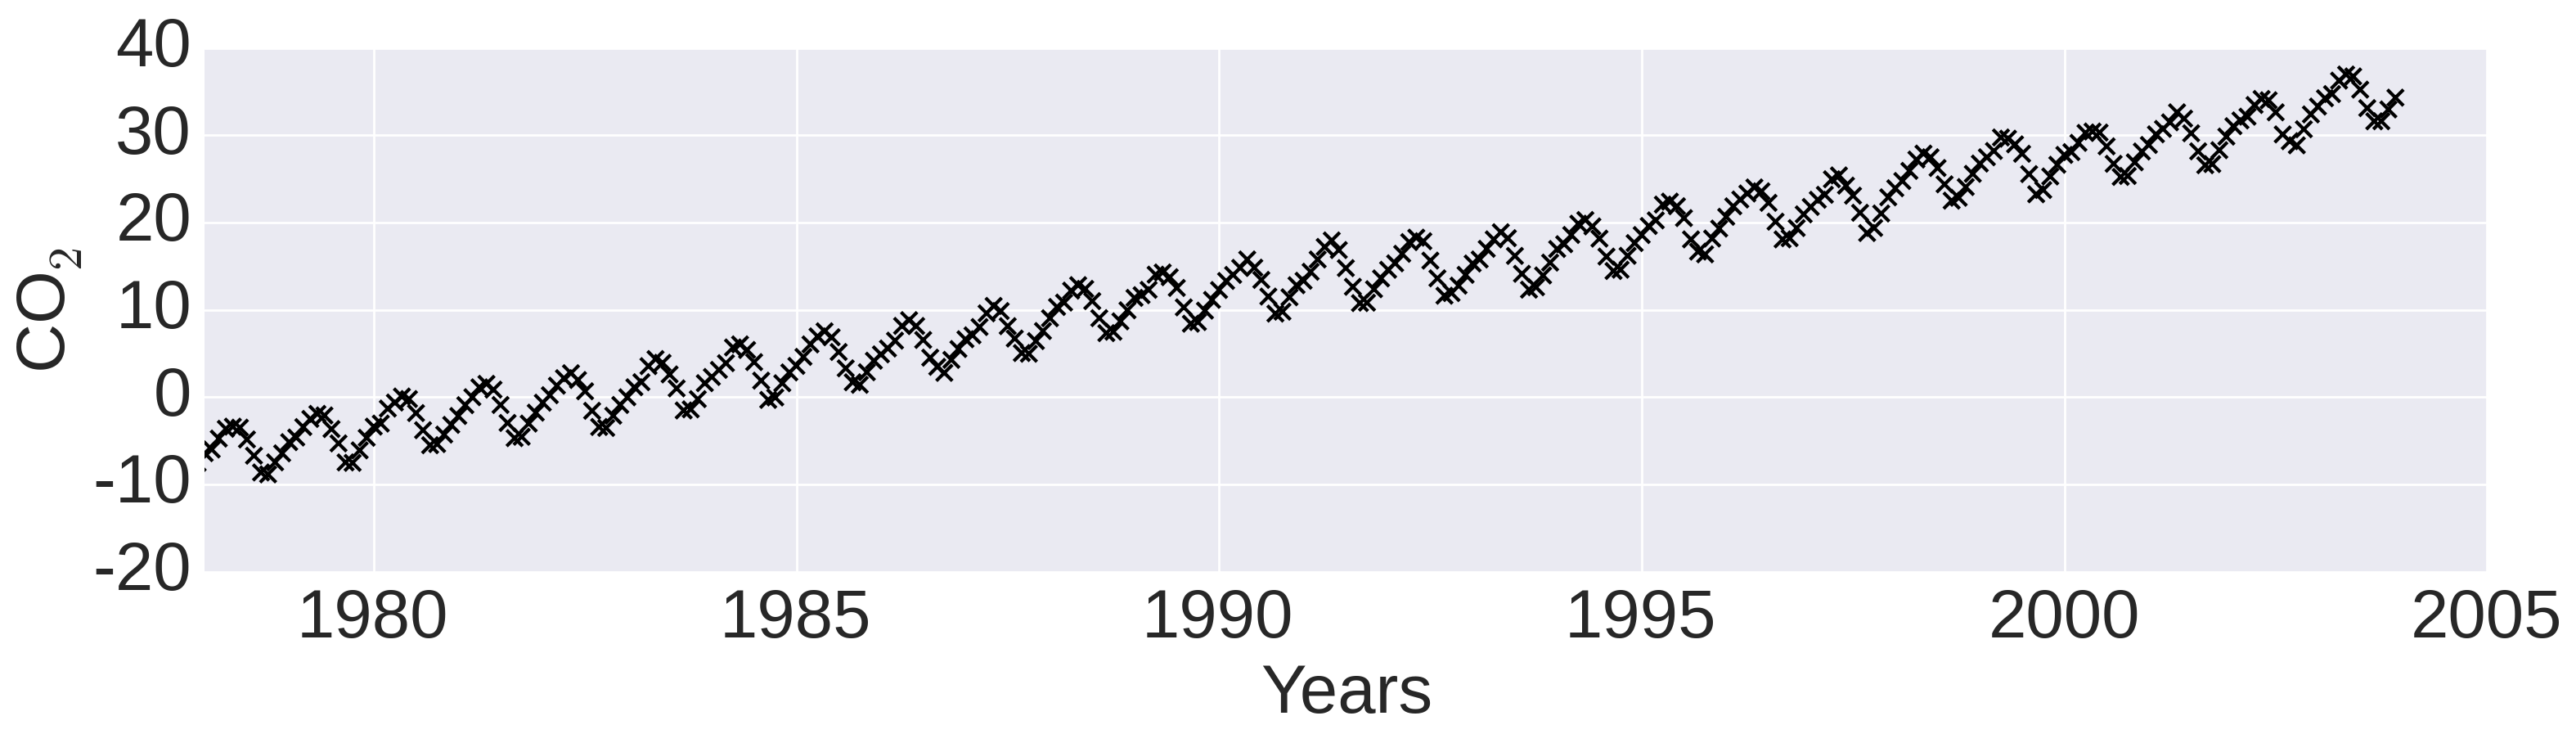
\includegraphics[width=0.7\textwidth]{figs/mauna_data.png}};
\node[below = 2.5cm of data] (post_param_helper) {};
\node[above = 1cm of post_param_helper] (post_param_helper_1) {};
\node[below = 1cm of post_param_helper] (post_param_helper_2) {};
\node[left = -3cm of post_param_helper] (post_param) {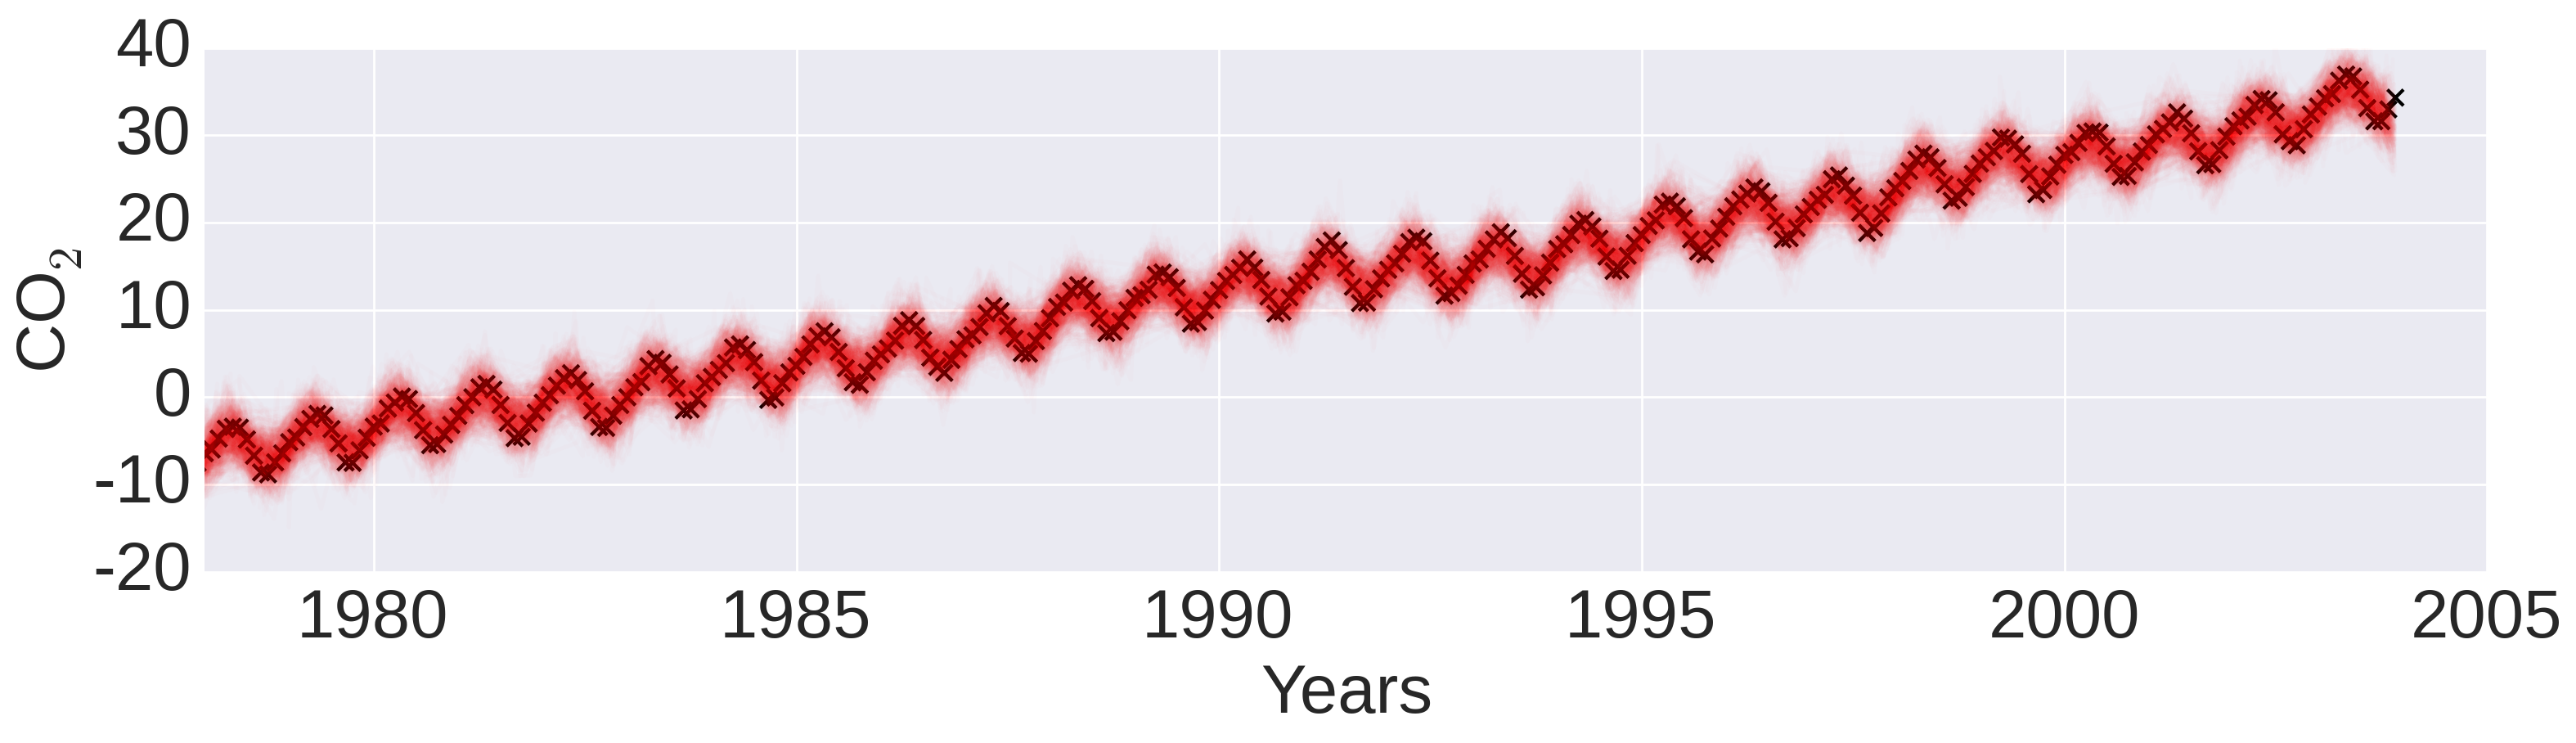
\includegraphics[width=0.6\textwidth]{figs/mauna_sample_1.png}};
\node[draw,rectangle,color=red,dashed,right = 4.5cm of post_param_helper,yshift=0.3cm] (zoom) {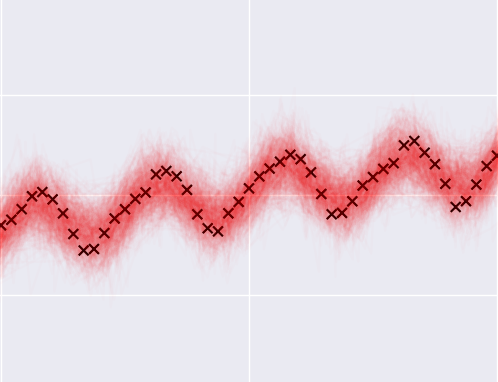
\includegraphics[width=0.2\textwidth]{figs/mauna_zoom.png}};
\node[draw,rectangle,color=red,dashed,left = 3.8cm of zoom, minimum width =
1.5cm, minimum height = 1.2cm,yshift=0.0cm] (zoom_in) {};
\node[below = 1.2cm of post_param_helper_2] (posterior) {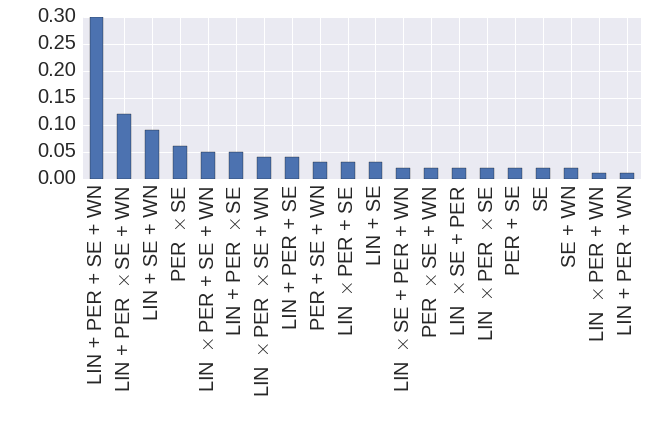
\includegraphics[width=0.6\textwidth]{figs/mauna_structure.png}};

\node[draw,rectangle,below = 1.2cm of posterior] (formula_param_1) {\color{black}\small
$\Ktheta= 2.7^2(x x^\prime) + 5.6^2 \exp \bigg( \frac{2 \sin^2 ( \pi (x - x^\prime)/3.7}{6.4^2} \bigg)
+ 0.4^2 \exp(-\frac{(x-x^\prime)^2}{2 \times 6.3^2}) +  1.9^2 \delta_{x,x^\prime} \label{eq:WN}$ };


\node[draw,rectangle,below = 1.2cm of formula_param_1,text width =
0.9\textwidth,minimum height = 1.5cm,font=\footnotesize] (paragraph){
The posterior peaks at a kernel structure with four additive components. Additive components hold globally, that is there are no higher level, qualitative aspects of the data that vary with the input space. The additive components are as follows: (i) a linearly increasing function or trend; (ii) a periodic function; (iii) a smooth function; and (iv) white noise.};







\node[draw, rectangle, left = -1.75cm of posterior,minimum width = 0.45cm, minimum height = 5.8cm,yshift=0.2cm] (mark_structure) {};
%\node[draw,very thick, rectangle, below = 1.1cm of data,minimum width = \textwidth, minimum height = 15cm] (posterior_frame) {};

%\node[left = 1.3cm of mark_structure] (paragraph_helper){};
\node[below =0.45cm of mark_structure,inner sep = 0pt,outer sep=0pt] (formula_helper) {};
\node[above =1.2cm of formula_param_1,inner sep = 0pt,outer sep=0pt] (formula_helper_2) {};

%\draw[-,dashed] (mark_structure.south) -- (formula_helper);
%\draw[-,dashed] (formula_helper) -- (formula_helper_2);
%\draw[->,dashed] (mark_structure) -- (paragraph_helper);
%\draw[->,dashed] (formula_helper_2) -- (formula);

\draw[->] (data) -- node[right]{\small $\hat \fbf \sim
\mathcal{N}(\hat{\bm{\mu}},\hat\Kbf)$} (post_param_helper_1);
\draw[->] (post_param_helper_2) -- node[right]{\small Marginal Structure} (posterior);
\draw[->] (formula_helper_2) -- node[right] {\small
$\bm{\theta}=\{2.7,5.6,3.7,6.4,0.4,6.3,1.9\}$} (formula_param_1);
\draw[-] (mark_structure) -- node[left, yshift=-0.3cm] {\small $\Ktheta$} (formula_helper);
\draw[-] (formula_helper) --(formula_helper_2);
\draw[->] (formula_param_1) -- node[right]{\small Qualitative Interpretation} (paragraph);

\draw[->,dashed,red] (zoom_in) --node[above]{\small\color{red}Zoom in:}
node[below]{\small\color{red}adequate error bars}(zoom);

%\draw[->,line width=1pt,double distance=2pt] (data) -- (post_param);
% starting from the bottom to aligm with caption 
\node[left=0.3cm of paragraph] (e){(e)}; 

\node[above=1.9cm of e] (d) {(d)}; 
\node[above=5.0cm of d] (c) {(c)}; 
\node[above=4.7cm of c] (b) {(b)}; 
\node[above=4.0cm of b] (a) {(a)}; 
\end{tikzpicture}
\addtolength\abovedisplayskip{1\baselineskip}%
\addtolength\belowdisplayskip{1\baselineskip}%


